\documentclass[hyperref={pdfpagelabels=true},ucs]{beamer}

%\usetheme{Warsaw}
\usetheme{GSyC}


%\usebackgroundtemplate{\includegraphics[width=\paperwidth]{../format/blank-bg.png}}


\usepackage[spanish]{babel}
\usepackage[utf8x]{inputenc}
\usepackage[T1]{fontenc}
\usepackage{upquote}

\usepackage{graphics}
\usepackage{amssymb} % Simbolos matematicos
\usepackage{fancyvrb}
\usepackage{multicol}
\usepackage{tikz}
\usetikzlibrary{arrows,shapes,backgrounds}

 \tikzset{
     %Define standard arrow tip
     >=stealth',
     %Define style for boxes
     punkt/.style={
            rectangle,
            rounded corners,
            draw=black, very thick,
            text centered},
     % Define arrow style
     pil/.style={
            ->,
            thick,
            shorten <=2pt,
            shorten >=2pt,}
}


\fvset{frame=single,commandchars=\\\{\}}

\definecolor{darkred}{rgb}  {0.7, 0.0, 0.15}
\definecolor{darkgreen}{rgb}{0.0, 0.4, 0.0}
\definecolor{darkblue}{rgb} {0.0, 0.0, 0.5}


% for resalted text
\newcommand{\res}[1]{\textcolor{darkred}{#1}}
% for different text
\newcommand{\dif}{\textsl}
% for reserved words
\newcommand{\rw}[1]{\textrm{\textbf{#1}}}
% for commands
\newcommand{\com}[1]{\textrm{\textbf{#1}}}



%% Metadatos del PDF.
\hypersetup{
  pdftitle={HTTP},
  pdfauthor={GSyC},
  pdfcreator={GSyC},
  pdfproducer=PDFLaTeX,
  pdfsubject={Sistemas Telemáticos para Medios Audiovisuales},
}
%%


%\pgfdeclareimage[height=0.5cm]{gsyc-logo}{../format/gsyc}
%\logo{\pgfuseimage{gsyc-logo}}



\AtBeginSection[]
{
  \begin{frame}<beamer>[shrink=25]{Contenidos}
    \tableofcontents[currentsection,hideallsubsections]
  \end{frame}
}

\AtBeginSubsection[]
{
  \begin{frame}<beamer>{Contenidos}
    \tableofcontents[currentsection,currentsubsection]
  \end{frame}
}




\begin{document}

%% Entre corchetes como argumento opcional un título o autor abreviado
%% para los pies de transpa

\title{HTTP}
\subtitle{Sistemas Telemáticos para Medios Audiovisuales}
%\institute{gsyc-profes@gsyc.escet.urjc.es}
\author[GSyC]{GSyC\\Departamento de Teoría de la Señal y Comunicaciones y Sistemas Telemáticos y Computación}
\date[2015]{Noviembre de 2015}

\frame{
\titlepage
\begin{center}
%\includegraphics[width=2cm]{../format/gsyc}
\end{center}
}




%% LICENCIA DE REDISTRIBUCIÓN DE LAS TRANSPAS
\frame{
~
\vspace{4cm}
\begin{flushright}
{\tiny
\copyright 2015 Grupo de Sistemas y Comunicaciones. \\
  Algunos derechos reservados. \\
  Este trabajo se distribuye bajo la licencia \\
  Creative Commons Attribution Share-Alike\\
  disponible en http://creativecommons.org/licenses/by-sa/3.0/es\\
}
\end{flushright}
}
%%
%%%%%%%%%%%%%%%%%%%%%%%%%%%%%%%%%%%%%%%%%%%%%%%%%%%%%%%%%%%%%%%%%%%

\begin{frame}[shrink=25]
  \frametitle{Contenidos}
  \tableofcontents[hideallsubsections]
\end{frame}


%\tikzstyle{every picture}+=[remember picture]
%\tikzstyle{na} = [baseline=-.5ex]

%%%%%%%%%%%%%%%%%%%%%%%%%%%%%%%%%%%%%%%%%%%%%%%%%%%%%%%%%%%%%%%%%%%
\section{Introducción}
%%%%%%%%%%%%%%%%%%%%%%%%%%%%%%%%%%%%%%%%%%%%%%%%%%%%%%%%%%%%%%%%%%%

\begin{frame}
\frametitle{Definiciones}

\begin{block}{URL \emph{(Universal Resource Locator)}}
Interfaz común para acceder a diferentes tipos de servicios/documentos
en Internet a través de un sistema de nombres.
\end{block}

\begin{block}{HTML \emph{(HyperText Markup Language)}}
Lenguaje de marcado para la elaboración de contenidos integrados por
texto, gráficos, etc, que permite incluir en un documento referencias
a otros recursos mediante URLs
\end{block}


\begin{block}{HTTP \emph{(HyperText Transfer Protocol)}}
Protocolo entre navegadores y servidores WWW para transferir
recursos hipermedia (texto, gráficos, audio, vídeo).
\end{block}

\end{frame}




%%%%%%%%%%%%%%%%%%%%%%%%%%%%%%%%%%%%%%%%%%%%%%%%%%%%%%%%%%%%%%%%%%%

\begin{frame}
\frametitle{URL}

\begin{center}
\includegraphics[width=90mm]{figs/newfigs-p01}
\end{center}

\begin{itemize}
\item \res{Protocolo}: Protocolo por el que se accede al recurso. Por
  defecto el predeterminado para la aplicación que usa la URL.
\item \textcolor{darkblue}{Máquina}: Máquina en la que reside el recurso. Por defecto la
  máquina local.
\item \textcolor{darkgreen}{Puerto}: Puerto de la máquina a través del que se pide el
  recurso. Por defecto el predeterminado para el protocolo (http=80)
\item \textcolor{violet}{Recurso}: Identificación del recurso dentro de la máquina,
  incluyendo (a veces) un \emph{path}. Por defecto el recurso
  predeterminado para la máquina.
\item \textcolor{orange}{Identificador de fragmento}: Opcionalmente, se utiliza para
  identificar un fragmento del recurso.
\end{itemize}
\end{frame}





%%%%%%%%%%%%%%%%%%%%%%%%%%%%%%%%%%%%%%%%%%%%%%%%%%%%%%%%%%%%%%%%%%%

\begin{frame}[fragile]
\frametitle{HTML}

~\hspace{-5mm}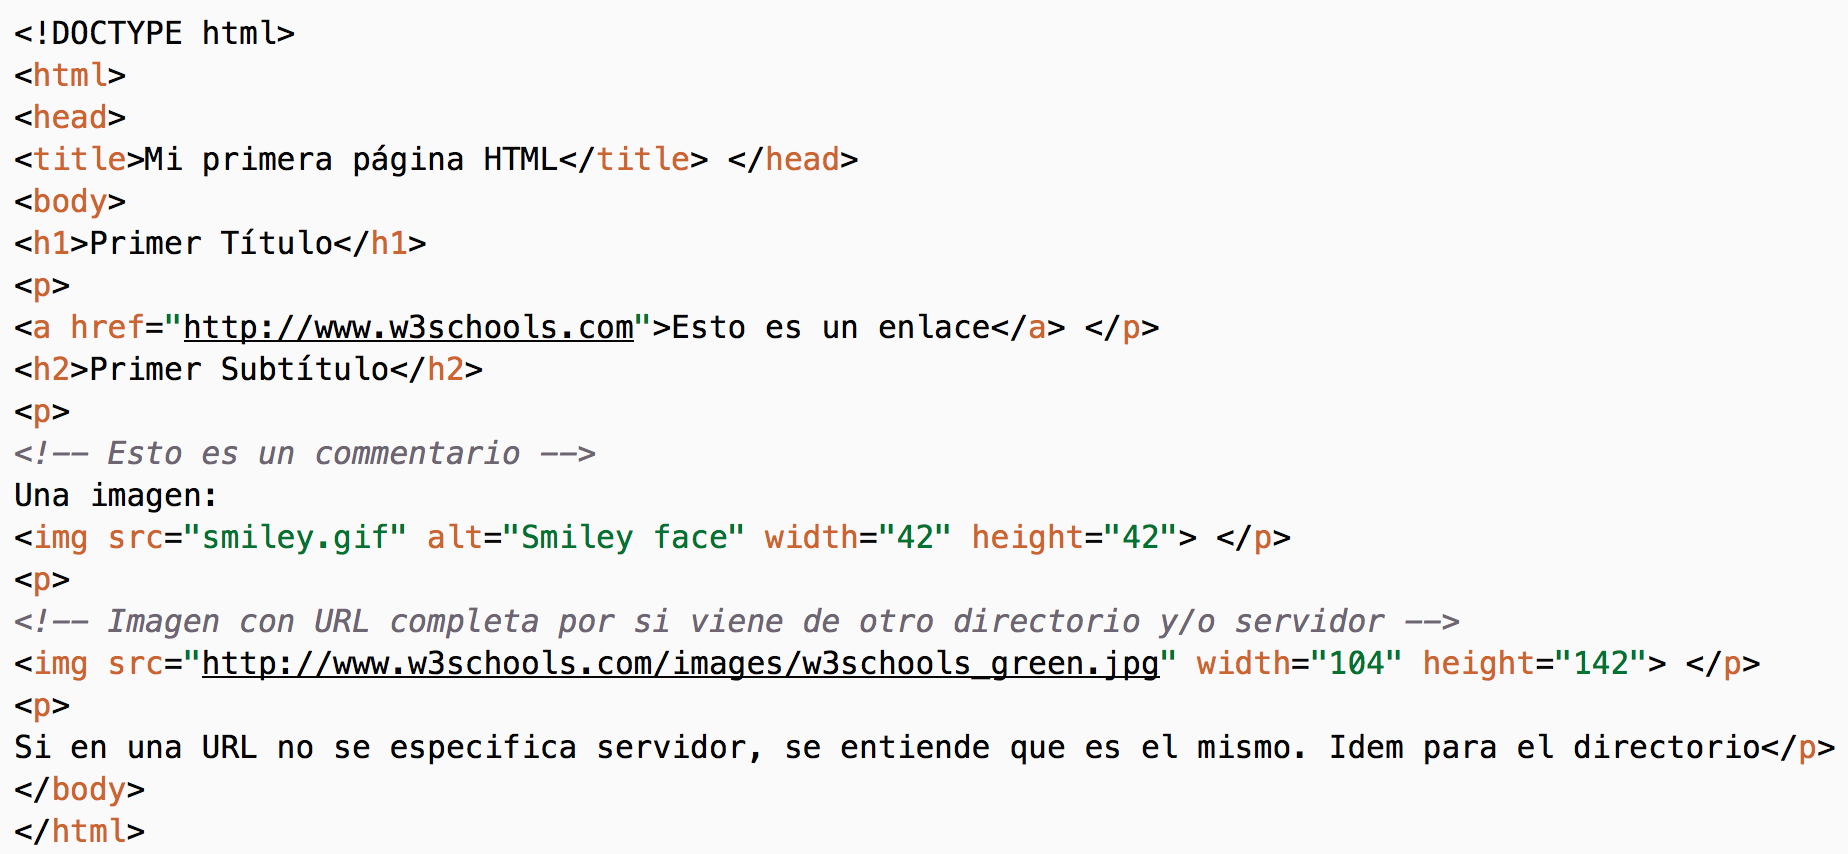
\includegraphics[width=1.1\textwidth]{figs/html-sample}



% \begin{tiny}
% \begin{verbatim}
% <!DOCTYPE html>
% <html>
% <head>
% <title>Mi primera página HTML</title>
% </head>

% <body>
% <h1>Primer Título</h1>

% <p>
% <a href="http://www.w3schools.com">Esto es un enlace</a>
% </p>

% <h2>Primer Subtítulo</h2>

% <p>
% <!-- Esto es un commentario -->
% Una imagen:
% <img src="smiley.gif" alt="Smiley face" width="42" height="42">
% </p>

% <p>
% <!-- Imagen con URL completa por si viene de otro directorio y/o servidor -->
% <img src="http://www.w3schools.com/images/w3schools_green.jpg" width="104" height="142">
% </p>

% <p>
% Si en una URL no se especifica servidor, se entiende que es el
% mismo. Idem para el directorio</p>
% </body>
% </html>
% \end{verbatim}
% \end{tiny}


\end{frame}

%%%%%%%%%%%%%%%%%%%%%%%%%%%%%%%%%%%%%%%%%%%%%%%%%%%%%%%%%%%%%%%%%%%

\begin{frame}
\frametitle{Visor de HTML}

\begin{center}
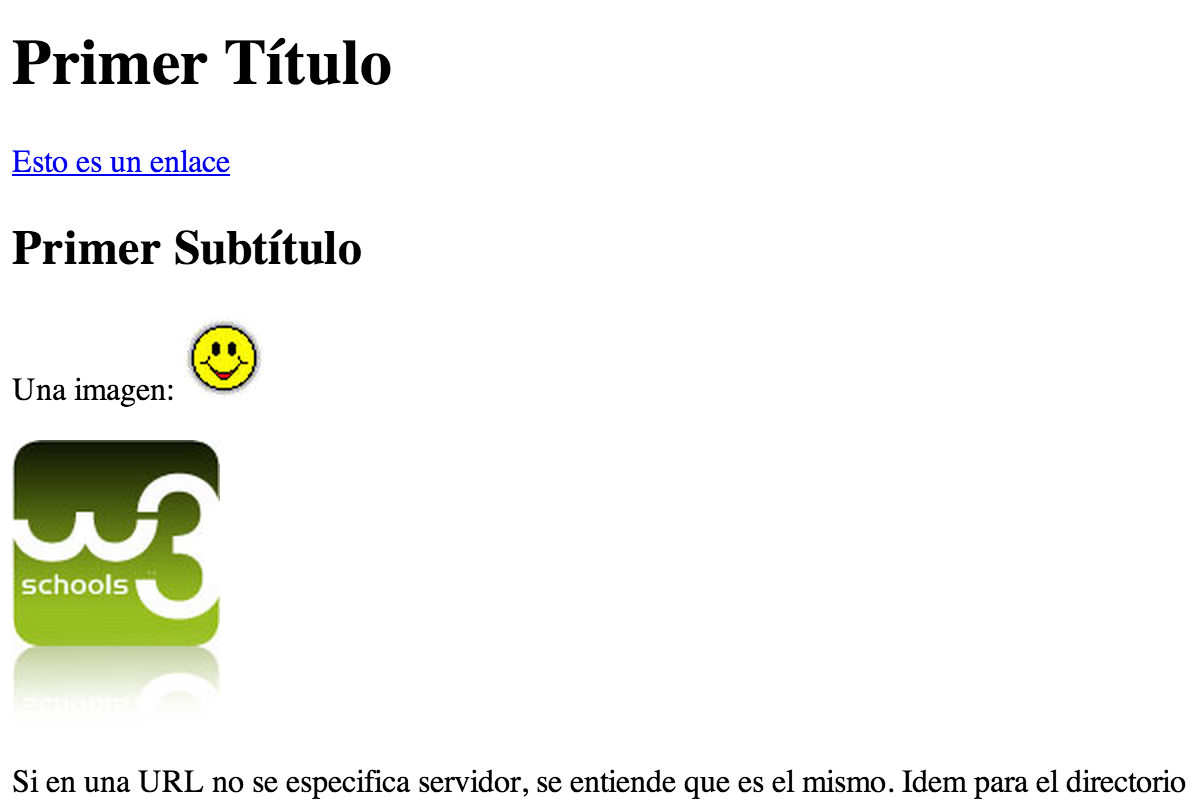
\includegraphics[width=90mm]{figs/html-example}
\end{center}

\end{frame}




%%%%%%%%%%%%%%%%%%%%%%%%%%%%%%%%%%%%%%%%%%%%%%%%%%%%%%%%%%%%%%%%%%%

\begin{frame}
\frametitle{HTTP}

\begin{columns}[l]

\column{35mm}

\begin{center}
\includegraphics[height=30mm]{figs/http-torre}
\end{center}

\column{90mm}

\begin{itemize}
\item Protocolo de nivel de aplicación utilizado para transferir
  recursos hipermedia entre ordenadores.
\item Sigue el \res{modelo Cliente-Servidor}:
  \begin{itemize}
  \item \textbf{Cliente HTTP}: navegador web que pide páginas y, al recibirlas, las
    muestra al usuario. Ej: Firefox, Explorer, Chrome, Safari\ldots
  \item \textbf{Servidor HTTP}: servidor web en el que están alojadas páginas que
    piden los clientes. Ej: Apache, IIS\ldots
  \end{itemize}
\item Funciona sobre TCP como protocolo de transporte
\item Por defecto un servidor HTTP escucha en el puerto 80, pero puede
  usar cualquier otro puerto.
\item HTTP puede servir tanto \res{contenido estático} (ficheros) como
  \res{contenido dinámico} (el resultado de ejecutar programas en el
  servidor).
\end{itemize}

\end{columns}

\end{frame}




%%%%%%%%%%%%%%%%%%%%%%%%%%%%%%%%%%%%%%%%%%%%%%%%%%%%%%%%%%%%%%%%%%%

\begin{frame}
\frametitle{Versiones de HTTP}

\begin{itemize}
\item \res{0.9}: Primera versión documentada, no tiene número de
  versión oficial, pero es referida como versión 0.9 (1991)
\item \res{1.0}: Primera versión oficial (RFC 1945, año 1996)
\item \res{1.1}: Versión ``clásica'' (RFC 2068, año 1997 y RFC 2616, año 1999)
\item \res{2.0}: Versión ``nueva'' (RFC 7540, junio 2015)
  \begin{itemize}
  \item Soportado en las versiones actuales de todos los navegadores
  \item Soportado por el 2\% de los servidores HTTP actuales (según
    W$^3$Tech)
  \end{itemize}
\end{itemize}


\end{frame}




%%%%%%%%%%%%%%%%%%%%%%%%%%%%%%%%%%%%%%%%%%%%%%%%%%%%%%%%%%%%%%%%%%%
\section{Relación entre HTTP y conexiones TCP}
%%%%%%%%%%%%%%%%%%%%%%%%%%%%%%%%%%%%%%%%%%%%%%%%%%%%%%%%%%%%%%%%%%%


%%%%%%%%%%%%%%%%%%%%%%%%%%%%%%%%%%%%%%%%%%%%%%%%%%%%%%%%%%%%%%%%%%%


\begin{frame}
\frametitle{Páginas web}

\begin{itemize}
\item Una \textbf{página web} se compone de uno o más \res{recursos}.
\item Cada recurso suele ser un archivo, y hay recursos de distinto
  tipo (archivos HTML, imágenes PNG, vídeos AVI, applets Java, etc)
\item A un recurso se hace referencia a través de su URL.
\item La mayoría de las páginas web están formadas por \res{un archivo HTML
  base y varios recursos referenciados} dentro de ese archivo base como
  contenido adicional de la misma página.
  \begin{itemize}
  \item Ej: Una página web puede estar compuesta por 6 recursos: 1
    fichero HTML y 5 imágenes PNG.
  \end{itemize}

\end{itemize}

\end{frame}



%%%%%%%%%%%%%%%%%%%%%%%%%%%%%%%%%%%%%%%%%%%%%%%%%%%%%%%%%%%%%%%%%%%%

\begin{frame}[shrink=10]
\frametitle{Petición de una página web de un sólo recurso}

\begin{center}
\includegraphics[height=6cm]{figs/tpo-1-rec}
\end{center}

\begin{itemize}
\item El tiempo total mide lo que se tarda en tener el recurso en el
  cliente (para mostrarlo, p.ej), por lo que el tiempo de cerrar la
  conexión no cuenta.
\end{itemize}


% \item NOTA: El protocolo HTTP \res{no mantiene estado}: un servidor
%   trata cada petición HTTP de manera aislada, sin almacenar
%   información sobre las peticiones previas hechas por un mismo
%   cliente.
%     \begin{itemize}
%       \begin{scriptsize}
%       \item con frecuencia las aplicaciones web sí necesitan
%         guardar estado, ya veremos cómo lo hacen
%       \end{scriptsize}
%     \end{itemize}
% \end{itemize}


\end{frame}



%%%%%%%%%%%%%%%%%%%%%%%%%%%%%%%%%%%%%%%%%%%%%%%%%%%%%%%%%%%%%%%%%%%%

\begin{frame}[shrink=10]
\frametitle{Una página con 5 recursos: Conexiones NO Persistentes}

\begin{center}
\includegraphics[width=\textwidth]{figs/tpo-no-pers}
\end{center}

\begin{itemize}
\item Una vez que el cliente tiene el recurso principal, lo analiza y
  abre con el servidor conexiones en paralelo con la actual para pedir
  los 4 recursos adicionales.
\end{itemize}


\end{frame}


%%%%%%%%%%%%%%%%%%%%%%%%%%%%%%%%%%%%%%%%%%%%%%%%%%%%%%%%%%%%%%%%%%%%

\begin{frame}[shrink=10]
\frametitle{Una página con 5 recursos: Conexiones Persistentes}

\begin{center}
\includegraphics[width=\textwidth]{figs/tpo-pers}
\end{center}

\begin{itemize}
\item Una vez que el cliente tiene el recurso principal, lo analiza y
  pide por la misma conexión los 4 recursos adicionales, que se envían
  en paralelo.
\item Es 1 RTT más rápido que con conexiones persistentes.
\end{itemize}


\end{frame}


%%%%%%%%%%%%%%%%%%%%%%%%%%%%%%%%%%%%%%%%%%%%%%%%%%%%%%%%%%%%%%%%%%%%

\begin{frame}[shrink=10]
\frametitle{Conexiones Persistentes con recursos en servidores diferentes} 

\begin{center}
\includegraphics[width=\textwidth]{figs/tpo-pers-varios-serv}
\end{center}

\begin{itemize}
\item En cuanto al menos un recurso adicional esté en otro servidor
  será imprescidible abrir una nueva conexión, lo que introduce el RTT
  adicional.
\end{itemize}


\end{frame}





%%%%%%%%%%%%%%%%%%%%%%%%%%%%%%%%%%%%%%%%%%%%%%%%%%%%%%%%%%%%%%%%%%%%%%%%%%%%%%

\begin{frame}[fragile]
\frametitle{Detalles del tiempo de respuesta de un recurso HTTP}


\vspace{-3mm}
\begin{center}
\includegraphics[width=0.7\textwidth]{figs/newfigs-p03}
\end{center}

\begin{itemize}
\item \res{\textbf{Búsqueda en el DNS}}: Depende del RTT de acceso al servidor de
  DNS de la máquina, y del tiempo que tarda en encontrar la respuesta
  el servidor de DNS.
\item \textcolor{darkblue}{\textbf{Establecimiento de la conexión TCP}}: Depende del RTT de
  acceso al servidor web.
\item \textcolor{darkgreen}{\textbf{Solicitud de HTTP}}: Depende del RTT de
  acceso al servidor web.
\item \textbf{Respuesta de HTTP}: Depende del ancho de banda entre
  el cliente y el servidor web. Si el recurso es grande, este tiempo
  es el más grande, si el recurso es pequeño, este tiempo es el más
  pequeño. 

\end{itemize}



\end{frame}



%%%%%%%%%%%%%%%%%%%%%%%%%%%%%%%%%%%%%%%%%%%%%%%%%%%%%%%%%%%%%%%%%%%%%%%%%%%%%%

\begin{frame}[fragile,shrink=5]
\frametitle{Tiempo de carga de página: Ingeniería de ``usabilidad''}

\begin{block}{Tiempo de carga de página (\emph{Page Load Time})}
Tiempo desde que el usuario hace clic en un enlace hasta que ve la
página pedida ``razonablemente'' completa.
\end{block}


\begin{center}
  \begin{tabular}{|c|c|}\hline
    \res{\textbf{Tiempo}} & \res{\textbf{Reacción del usuario}} \\\hline
    0 - 100 ms & carga instantánea \\   
    100 - 300 ms & sensación de lentitud \\   
    300 - 1000 ms & espera apreciable \\   
    1 - 10 s & cambio de contexto mental \\   
    $>$ 10 s & abandono de la página \\\hline 
  \end{tabular}
\end{center}

\begin{itemize}
\item Se considera importante mantenerse por debajo de los 
  \res{250 ms} para que la navegación sea fluida.
\item Valores experimentales medios a día de hoy:
  \begin{itemize}
  \item RTT: 100 ms
  \item Tiempo de carga de página: 7 s (mediana: 3 s)
  \end{itemize}
\item Valores aún peores usando dispositivos móviles.
\end{itemize}


\end{frame}




%%%%%%%%%%%%%%%%%%%%%%%%%%%%%%%%%%%%%%%%%%%%%%%%%%%%%%%%%%%%%%%%%%%%%%%%%%%%%%

\begin{frame}[fragile]
\frametitle{Tiempo de carga de página: cómo mejorarlo}

\vspace{-3mm}
\begin{center}
\includegraphics[width=\textwidth]{figs/newfigs-p02}
\end{center}

\begin{itemize}
\item El tiempo de carga de página depende sobre todo del RTT, y no
  tanto del ancho de banda.
\item El RTT depende de la latencia, no del ancho de banda
  (básicamente, RTT $=$ 2 $*$ latencia)
\item A día de hoy, mejorar el ancho de banda ya no mejora el tiempo
  de carga de la página. Hay que trabajar en el RTT:
  \begin{itemize}
  \item reduciendo la latencia
  \item minimizando el número de RTTs necesarios para cargar la página
  \end{itemize}
\end{itemize}

\end{frame}




%%%%%%%%%%%%%%%%%%%%%%%%%%%%%%%%%%%%%%%%%%%%%%%%%%%%%%%%%%%%%%%%%%%%%%%%%%%%%%

\begin{frame}[fragile]
\frametitle{Valores típicos en una aplicación web hoy}

Carga de la página principal de una aplicación web:
\begin{itemize}
\item 90 solicitudes de HTTP, obtenidas de 15 servidores, 1300 KB
  transferidos, 3 segundos:
  \begin{itemize}
  \item HTML: 10 solicitudes, 52 KB
  \item Imágenes: 55 solicitudes, 812 KB
  \item JavaScript: 15 solicitudes, 216 KB
  \item CSS: 5 solicitudes, 36 KB
  \item Otros: 5 solicitudes, 195 KB
  \end{itemize}
\end{itemize}

% \begin{center}
% \includegraphics[height=55mm]{figs/}
% \end{center}


\end{frame}











%%%%%%%%%%%%%%%%%%%%%%%%%%%%%%%%%%%%%%%%%%%%%%%%%%%%%%%%%%%%%%%%%%%
\section{Formato de mensajes HTTP}
%%%%%%%%%%%%%%%%%%%%%%%%%%%%%%%%%%%%%%%%%%%%%%%%%%%%%%%%%%%%%%%%%%%


%%%%%%%%%%%%%%%%%%%%%%%%%%%%%%%%%%%%%%%%%%%%%%%%%%%%%%%%%%%%%%%%%%%

\begin{frame}[fragile, shrink=25]
\frametitle{Formato general de los mensajes}


\begin{itemize}

\item Los clientes envían mensajes llamados \res{peticiones}
\item Los servidores envían mensajes llamados \res{respuestas}
\item Todos los mensajes tienen un \res{formato de texto}: Un mensaje es una
  colección de líneas de texto.
\item Cada \res{línea de texto} es un conjunto de caracteres terminado
  por un carácter especial ``fin de línea'' o por la pareja de
  caracteres \verb|<CR><LF>|.

\item Formato:

\vspace{-5mm}
\begin{center}
\includegraphics[width=\textwidth]{figs/formato-general}
\end{center}

\end{itemize}

\end{frame}

%%%%%%%%%%%%%%%%%%%%%%%%%%%%%%%%%%%%%%%%%%%%%%%%%%%%%%%%%%%%%%%%%%%



\begin{frame}[fragile]
\frametitle{Formato peticiones}

\begin{center}
\includegraphics[width=\textwidth]{figs/formato-peticiones}
\end{center}


\begin{itemize}

\item La especificación del recurso incluya la ruta (\emph{path}),
  pero no el nombre de máquina.
\item La versión del protocolo indica la versión que entiende el
  cliente.
\item Las peticiones normalmente no llevan cuerpo (aunque, a veces, sí).
\end{itemize}

\end{frame}


%%%%%%%%%%%%%%%%%%%%%%%%%%%%%%%%%%%%%%%%%%%%%%%%%%%%%%%%%%%%%%%%%%%



\begin{frame}[fragile, shrink=35]
\frametitle{Formato respuestas}

\begin{center}
\includegraphics[width=\textwidth]{figs/formato-respuestas}
\end{center}


\begin{itemize}
\item La versión del protocolo indica la mayor versión que entiende el
  servidor, pero siempre se responde atendiendo a la versión de la
  petición recibida.
\item Las respuestas normalmente sí llevan cuerpo: el recurso solicitado.
\end{itemize}

\end{frame}




%%%%%%%%%%%%%%%%%%%%%%%%%%%%%%%%%%%%%%%%%%%%%%%%%%%%%%%%%%%%%%%%%%%


\begin{frame}[fragile]
\frametitle{Respuestas: Resultado}

\begin{itemize}

\item Códigos de estado del resultado en los mensajes de respuesta:

  \begin{itemize}
  \item \res{1xx}: Mensaje informativo
  \item \res{2xx}: Resultado con éxito\\
    {\scriptsize \Verb|       200 OK|}
  \item \res{3xx}: Redirección del cliente a otra URL\\
    {\scriptsize \Verb|       301 Moved permanently|}
    permanently).
  \item \res{4xx}: Error en el lado del cliente\\
    {\scriptsize  \Verb|       404 Not Found|}
  \item \res{5xx}: Error en el lado del servidor\\
    {\scriptsize  \Verb|       500 Server Error|}
  \end{itemize}

\end{itemize}

\end{frame}


%%%%%%%%%%%%%%%%%%%%%%%%%%%%%%%%%%%%%%%%%%%%%%%%%%%%%%%%%%%%%%%%%%%


\begin{frame}[fragile,shrink=18]
\frametitle{Líneas de cabecera}


\begin{itemize}
\item Mismo formato que las cabeceras del formato de los correos
  electrónicos (RFC 822, sección 3).

\item En HTTP/1.0 se definen 16 cabeceras, ninguna obligatoria.

\item En HTTP/1.1 se definen 46 cabeceras, \textbf{siendo obligatoria
    en las peticiones la cabecera} \Verb|\textcolor{darkblue}{Host}|:
  nombre del servidor del recurso\\
    {\scriptsize \Verb|               Host: www.urjc.es|}

\item Se recomienda incluir en las peticiones al menos: 
  \begin{itemize}
  \item \Verb|\textcolor{darkblue}{User-Agent}|: tipo de navegador\\
    {\scriptsize \Verb|          User-Agent: Mozilla/5.0|}
  \end{itemize}

\item Se recomienda incluir en las respuestas al menos:
  \begin{itemize}
  \item \Verb|\textcolor{darkblue}{Server}|: tipo de servidor\\
    {\scriptsize \Verb|          Server: Apache/1.3|}
  \item \Verb|\textcolor{darkblue}{Last-Modified}|: fecha de última
    modificación del recurso\\
    {\scriptsize \Verb|          Last-Modified: Wed, 28 May 2014 18:41:38 GMT|}
  \end{itemize}

\item Si un mensaje tiene cuerpo, es obligatorio que se incluyan las
  cabeceras:
  \begin{itemize}
  \item \textcolor{darkblue}{\Verb|Content-Type|}: tipo MIME de lo que
    va en el cuerpo\\
    {\scriptsize \Verb|          Content-Type: text/html|}
  \item \textcolor{darkblue}{\Verb|Content-Length|}: tamaño en bytes
      del cuerpo\\
    {\scriptsize \Verb|          Content-Length: 10726|}
  \end{itemize}

\end{itemize}
\end{frame}

% %%%%%%%%%%%%%%%%%%%%%%%%%%%%%%%%%%%%%%%%%%%%%%%%%%%%%%%%%%%%%%%%%%%

% \begin{frame}[fragile]
% \frametitle{Otras Cabeceras}

% \begin{itemize}

% \item \textcolor{darkblue}{\Verb|Date|}: Fecha/hora de la operación
%     {\scriptsize \Verb|          Date: Tue, 10 Nov 2015 18:43:21 GMT|}

% \end{itemize}

% \end{frame}



%%%%%%%%%%%%%%%%%%%%%%%%%%%%%%%%%%%%%%%%%%%%%%%%%%%%%%%%%%%%%%%%%%%


\begin{frame}[fragile]
\frametitle{Cabecera para conexiones persistentes y no persistentes}

\begin{itemize}

\item En HTTP/1.0 las conexiones, por defecto, son no persistentes.
\item Si en HTTP/1.0 se quiere usar conexiones persistentes (los
  servidores no están obligados a soportarlas):
  \begin{enumerate}
  \item el cliente incluirá en su petición la cabecera
    \textcolor{darkblue}{\Verb|Connection: Keep-Alive|}
  \item si el servidor lo acepta incluirá en su respuesta la cabecera
    \textcolor{darkblue}{\Verb|Connection: Keep-Alive|}
  \end{enumerate}

\item En HTTP/1.1 y HTTP/2 las conexiones, por defecto son persistentes.
\item Si en HTTP/1.1 se quiere usar conexiones no persistentes:
  \begin{enumerate}
  \item el cliente incluirá en su petición la cabecera     
    \textcolor{darkblue}{\Verb|Connection: close|}
  \item el servidor incluirá en su respuesta la cabecera     
    \textcolor{darkblue}{\Verb|Connection: close|}
  \end{enumerate}

\end{itemize}


\end{frame}



%%%%%%%%%%%%%%%%%%%%%%%%%%%%%%%%%%%%%%%%%%%%%%%%%%%%%%%%%%%%%%%%%%%


\begin{frame}[fragile]
\frametitle{Métodos \texttt{GET} y \texttt{POST}}

\begin{itemize}
\item \textcolor{red}{\Verb|GET|}:
  \begin{itemize}
  \item Solicita un recurso al servidor especificando su URL.
  \end{itemize}

% \item \textcolor{red}{\Verb|HEAD|}:
%   \begin{itemize}
%   \item Igual que un GET, pero sólo pide las cabeceras.
%   \item Con este método se pueden consultar todas las cabeceras sin descargar el
%     recurso completo.
%     \begin{itemize}
%     \item Permite que los clientes puedan 
%       comprobar si ha habido modificaciones en un recurso sin
%       necesidad de transferirlo (para comparar, por ejemplo, si ha
%       habido modificiaciones frente a una versión en caché).
%     \end{itemize}
%   \end{itemize}

\item \textcolor{red}{\Verb|POST|}:
  \begin{itemize}
  \item Envía datos al servidor, normalmente los introducidos por el
    usuario en un formulario.
  \item Los datos van en el cuerpo.
  \item El \emph{path} de la línea inicial (URL) se refiere normalmente al programa
    que tratará los datos que se envian.
  \end{itemize}
  
\item \textbf{GET también permite enviar los datos de un
    formulario}. En este caso, los datos van en el \emph{path} de la
  línea inicial (URL), y no hay cuerpo. 
 
  \begin{itemize}
  \item El tamaño de los datos subidos con GET está limitado por el
    tamaño máximo de una URL (255 caracteres), por lo que NO~se
    utiliza GET para subir datos de formularios grandes.
  \end{itemize}

\end{itemize}

\end{frame}

%%%%%%%%%%%%%%%%%%%%%%%%%%%%%%%%%%%%%%%%%%%%%%%%%%%%%%%%%%%%%%%%%%%


\begin{frame}[fragile]
\frametitle{Ejemplo de formularios HTML}

\begin{itemize}
\item Formulario que enviará los datos mediante \Verb|GET|:
\begin{scriptsize}
\begin{Verbatim}
<FORM action="\textcolor{orange}{http://pc2.emp2.net/form.php}" method=\textcolor{red}{GET}>
   <P>
   Nombre: <INPUT type="text" name="\textcolor{red}{nombre}"><BR>
   Edad: <INPUT type="text" name="\textcolor{red}{edad}"><BR>
   <INPUT type="submit" value="Enviar"><INPUT type="reset">
   </P>
</FORM>
\end{Verbatim}
\end{scriptsize}

\item Formulario que enviará los datos mediante \Verb|POST|:
\begin{scriptsize}
\begin{Verbatim}
<FORM action="\textcolor{orange}{http://pc2.emp2.net/form.php}" method=\textcolor{red}{POST}>
   <P>
   Nombre: <INPUT type="text" name="\textcolor{red}{nombre}"><BR>
   Edad: <INPUT type="text" name="\textcolor{red}{edad}"><BR>
   <INPUT type="submit" value="Enviar"><INPUT type="reset">
   </P>
</FORM>
\end{Verbatim}
\end{scriptsize}

\end{itemize}

\end{frame}

%%%%%%%%%%%%%%%%%%%%%%%%%%%%%%%%%%%%%%%%%%%%%%%%%%%%%%%%%%%%%%%%%%%


\begin{frame}[fragile]
\frametitle{Ejemplo de envío de datos con \texttt{GET} y \texttt{POST}}

\begin{columns}[c]

\column{85mm}

\begin{scriptsize}
\begin{Verbatim}
\textcolor{red}{GET} \textcolor{orange}{/form.php}\textcolor{red}{?nombre=Fulano+Mengano&edad=24} HTTP/1.0
Host: pc2.emp2.net
User-Agent: Mozilla/4.5 [en]
Accept: image/jpeg, image/gif, text/html
Accept-language: en
Accept-Charset: iso-8859-1

\end{Verbatim}
\end{scriptsize}

\begin{scriptsize}
\begin{Verbatim}
\textcolor{red}{POST} \textcolor{orange}{/form.php} HTTP/1.0
Host: pc2.emp2.net
User-Agent: Mozilla/4.5 [en]
Accept: image/jpeg, image/gif, text/html
Accept-language: en
Accept-Charset: iso-8859-1
\textcolor{darkgreen}{Content-Type: application/x-www-form-urlencoded}
\textcolor{darkgreen}{Content-Length: 26}

\textcolor{red}{nombre=Perico+Palotes&edad=24}
\end{Verbatim}
\end{scriptsize}

\column{35mm}

\begin{scriptsize}
\begin{itemize}
\item[?:] separación entre el recurso y los parámetros
\item[=:] separación entre nombre del campo del formulario y su
  valor
\item[\&:] separación entre parámetros
\item[+:] espacio en blanco
\end{itemize}
\end{scriptsize}

\end{columns}


\end{frame}

%%%%%%%%%%%%%%%%%%%%%%%%%%%%%%%%%%%%%%%%%%%%%%%%%%%%%%%%%%%%%%%%%%%


\begin{frame}[fragile]
\frametitle{Otros métodos}

\begin{itemize}
\item \textcolor{red}{\Verb|PUT|}:
  \begin{itemize}
  \item Actualiza un recurso en el servidor (``sube'' una página web).   
  \item Hoy no se usa para este fin, pues las páginas WWW se colocan
    en los servidores por mecanismos externos a HTTP.
  \end{itemize}

\item \textcolor{red}{\Verb|DELETE|}:
  \begin{itemize}
  \item Elimina en el servidor el recurso especificado.
  \item También en desuso para este fin.
  \end{itemize}

% \item \textcolor{red}{LINK}:
%   \begin{itemize}
%   \item Crea en el servidor una relación entre documentos.
%   \end{itemize}

% \item \textcolor{red}{UNLINK}:
%   \begin{itemize}
%   \item Elimina del servidor una relación existente entre documentos.
%   \end{itemize}

\item \textcolor{red}{\ldots}

\end{itemize}

\end{frame}



%%%%%%%%%%%%%%%%%%%%%%%%%%%%%%%%%%%%%%%%%%%%%%%%%%%%%%%%%%%%%%%%%%%

\begin{frame}[fragile]
\frametitle{Páginas web dinámicas: Aplicaciones Web}

\begin{itemize}
\item Las URL ahora NO identifican un recurso almacenado en un fichero,
  sino que \res{el recurso pedido se crea dinámicamente}, ejecutándose un
  programa en el servidor.
\item En la URL se especifica el nombre del programa a ejecutar y
  puede incluir argumentos que se le pasan al programa.
\item Estos programas que se ejecutan en el servidor suelen estar
  escritos en lenguajes de \emph{scripting}: \emph{shell-scripts},
  PHP, Perl, Python, Ruby
\item El resultado de la ejecución de estos programas es una página
  web (o una parte de ella).
\end{itemize}

\end{frame}





%%%%%%%%%%%%%%%%%%%%%%%%%%%%%%%%%%%%%%%%%%%%%%%%%%%%%%%%%%%%%%%%%%%

\begin{frame}[fragile]
\frametitle{Aplicaciones web que siguen el API REST}

\begin{itemize}
\item \res{REST} es una forma de diseñar aplicaciones web que hace un uso de
  las URLs y de los métodos de HTTP totalmente diferente al prevista
  en el protocolo:
  \begin{itemize}
  \item Las URLs no referencian recursos consistentes en archivos, ni
    recursos generados dinámicamente, sino objetos (elementos,
    componentes) de una aplicación.
  \item Método GET: se invoca para consultar el estado de un objeto
  \item Método PUT: se invoca para modificar el estado de un objeto
  \item Método DELETE: se invoca para borrar un objeto
  \end{itemize}
\item Este API REST ha hecho que se vuelvan a utilizar los métodos PUT
  y DELETE, abandonados en el HTTP convencional.

\end{itemize}

\end{frame}





%%%%%%%%%%%%%%%%%%%%%%%%%%%%%%%%%%%%%%%%%%%%%%%%%%%%%%%%%%%%%%%%%%%


\begin{frame}[fragile]
\frametitle{Usando HTTP desde \texttt{telnet}}

\begin{enumerate}
\item En un terminal, se realiza un \Verb|telnet| al puerto 80 de la
  máquina del servidor:
  \begin{columns}
    \column{60mm}
    \begin{scriptsize}
      \begin{Verbatim}
telnet www.urjc.es 80        
      \end{Verbatim}
    \end{scriptsize}
    \column{60mm}
    \begin{scriptsize}
      Abre una conexión TCP con el puerto 80 de \Verb|www.urjc.es|.
      Cualquier cosa que se teclee se enviará por la conexión.
    \end{scriptsize} 
  \end{columns}

\vspace{5mm}  
\item En un terminal, se realiza un \Verb|telnet| al puerto 80 de la
  máquina del servidor:
  \begin{columns}
    \column{60mm}
    \begin{scriptsize}
      \begin{Verbatim}
GET /index.html HTTP/1.0

      \end{Verbatim}
    \end{scriptsize}
    \column{60mm}
    \begin{scriptsize}
      Envía una petición de la página \Verb|index.html|. Es necesario
      dejar una línea en blanco para terminar la cabera HTTP.
    \end{scriptsize} 
  \end{columns}

\vspace{5mm}  
\item Se muestra la respuesta recibida del servidor.
\end{enumerate}

\end{frame}

%%%%%%%%%%%%%%%%%%%%%%%%%%%%%%%%%%%%%%%%%%%%%%%%%%%%%%%%%%%%%%%%%%%



%%%%%%%%%%%%%%%%%%%%%%%%%%%%%%%%%%%%%%%%%%%%%%%%%%%%%%%%%%%%%%%%%%%
\begin{frame}
\frametitle{Ejemplo de HTTP desde telnet}

\begin{center}
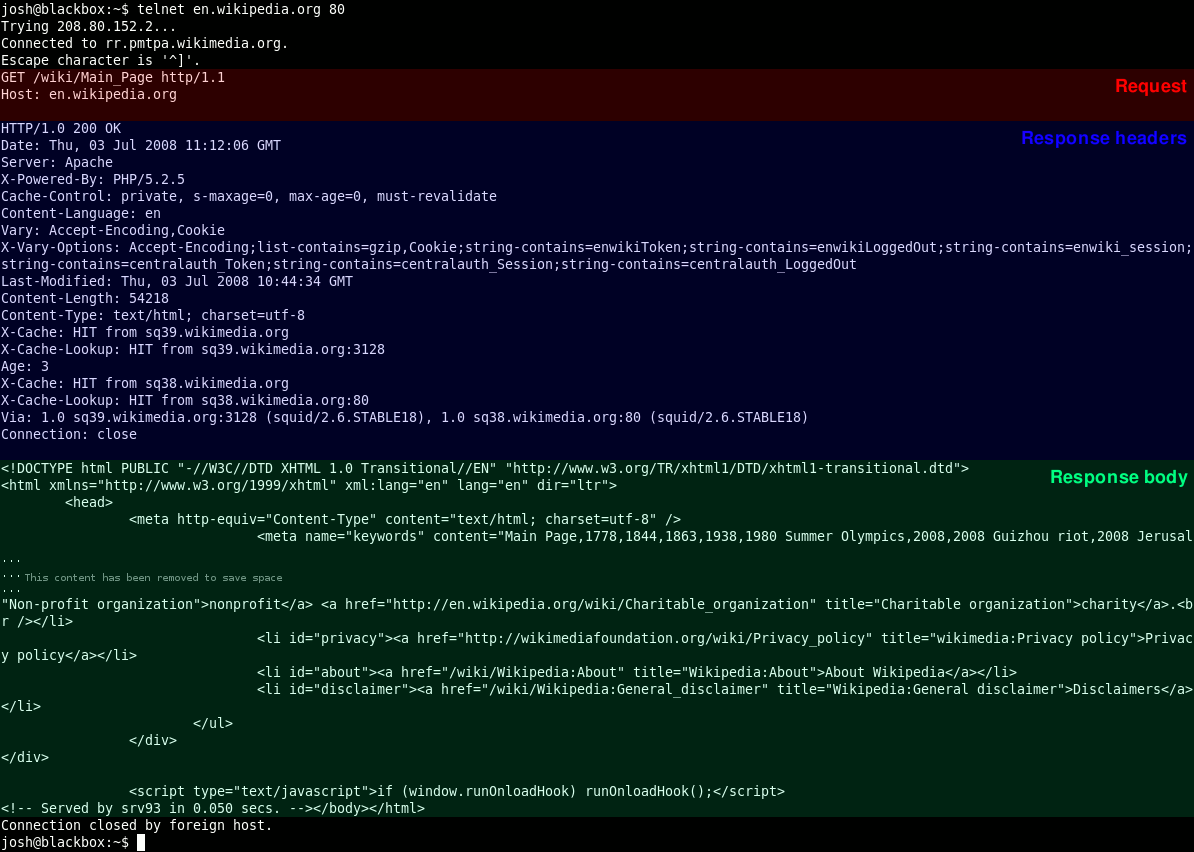
\includegraphics[width=\textwidth]{figs/http_request_telnet_ubuntu}  
\end{center}


\end{frame}



%%%%%%%%%%%%%%%%%%%%%%%%%%%%%%%%%%%%%%%%%%%%%%%%%%%%%%%%%%%%%%%%%%%
\section{Caché de contenidos en HTTP}
%%%%%%%%%%%%%%%%%%%%%%%%%%%%%%%%%%%%%%%%%%%%%%%%%%%%%%%%%%%%%%%%%%%

\begin{frame}[fragile,shrink=12]
\frametitle{Cachés en HTTP (I)}


\begin{block}{Objetivo}
Que un servidor no tenga que volver a enviar a un
  mismo cliente un mismo recurso que no ha cambiado.
\end{block}

\begin{itemize}
\item Cuando un cliente pide a un servidor un recurso por primera vez, se
  lo guarda en una caché (normalmente en disco).
\item El cliente guarda cada recurso en su caché junto
  con la \res{fecha de última modificación} del recurso y su \res{fecha de
  expiración} (que indica hasta cuándo se considera que el contenido del
  recurso es válido).

  \begin{itemize}
  \item El servidor envía el recurso indicando su fecha de última
    modificación, con la cabecera \Verb|\textcolor{blue}{Last-Modified: <fecha>}|
  \item El servidor puede fijar la fecha de expiración del recurso con
    la cabecera \Verb|\textcolor{blue}{Expires: <fecha>}|.
  \item Si el servidor no envía la cabecera \Verb|Expires|, el cliente
    calcula una fecha de expiración de forma directamente
    proporcional a la diferencia entre la fecha actual y la fecha de
    última modificación: cuanto más tiempo haga de la fecha de última
    modificación, más grande será la fecha de expiración.
  \end{itemize}

\end{itemize}
\end{frame}


%%%%%%%%%%%%%%%%%%%%%%%%%%%%%%%%%%%%%%%%%%%%%%%%%%%%%%%%%%%%%%%%%%%


\begin{frame}[fragile]
\frametitle{Cachés en HTTP (II)}


\begin{itemize}
\item Cuando un cliente quiere pedir un recurso a un servidor, primero
  comprueba si ya tiene dicho recurso en su caché, dentro de su
  periodo de vigencia:
  \begin{itemize}
  \item \res{Si NO está en la caché}, el cliente pide el recurso normalmente
    al servidor, y cuando lo tenga lo guardará en su caché.
  \item \res{Si SÍ está en la caché, y NO ha expirado}, el cliente no pide
    el recurso al servidor, sino que lo recupera de la caché.
  \item \res{Si SÍ está en la caché, y SÍ ha expirado}, el cliente lo
    pide al servidor con la cabecera 
    \Verb|\textcolor{blue}{If-modified-since: <fecha>}|, indicando la fecha de última
    modificación del recurso.
    \begin{itemize}
    \item Si el objeto NO ha cambiado en el servidor, el servidor
      responde un una respuesta \Verb|\textcolor{red}{304 Not Modified}|, sin enviar el recurso
    \item Si el objeto SÍ ha cambiado en el servidor, el servidor
      envía el recurso normalmente.
    \end{itemize}
  \end{itemize}

\end{itemize}


\end{frame}



%%%%%%%%%%%%%%%%%%%%%%%%%%%%%%%%%%%%%%%%%%%%%%%%%%%%%%%%%%%%%%%%%%%

\begin{frame}[fragile]
\frametitle{Cachés en HTTP (III)}

\begin{columns}[c]

\column{60mm}
\begin{itemize}
\item Objetivo: no enviar recursos si el cliente tiene una versión
  actualizada en su caché.

\item Cliente: especifica la fecha de la copia en caché en la petición HTTP:\\
\Verb|If-modified-since: <date>|

\item Servidor: su respuesta no contiene ningún recurso si no ha sido
  modificado desde la fecha especificada en la petición:\\
\Verb|HTTP/1.0 304 Not Modified|
\end{itemize}

\column{60mm}
\begin{center}
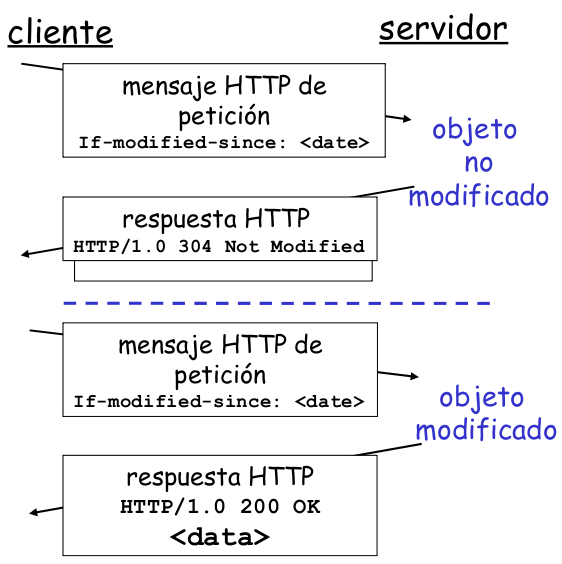
\includegraphics[width=60mm]{figs/5-p35}
\end{center}

\end{columns}

\end{frame}

%%%%%%%%%%%%%%%%%%%%%%%%%%%%%%%%%%%%%%%%%%%%%%%%%%%%%%%%%%%%%%%%%%%


% \begin{frame}[fragile]
% \frametitle{Otras condiciones}

% \begin{itemize}
% \item Los servidores deben responder siempre con la cabecera
%   \Verb|Date| indicando la fecha y hora actual (en GMT).

% \item Los servidores han de entender \Verb|If-Modified-Since| 
%y \Verb|If-Unmodified-Since|.

% \item Los clientes pueden usar o no usar \Verb|If-Modified-Since| 
%y \Verb|If-Unmodified-Since|.

% \item Respuesta a \Verb|If-Modified-Since|, si no se ha modificado el
%   recurso desde esa fecha: \verb|Not Modified|.

% \item Respuesta a \Verb|If-Unmodified-Since|, si se ha modificado el
%   recurso desde esa fecha: \Verb|Precondition Failed|.
% \end{itemize}

% \end{frame}


%%%%%%%%%%%%%%%%%%%%%%%%%%%%%%%%%%%%%%%%%%%%%%%%%%%%%%%%%%%%%%%%%%%
\section{Proxies de HTTP}
%%%%%%%%%%%%%%%%%%%%%%%%%%%%%%%%%%%%%%%%%%%%%%%%%%%%%%%%%%%%%%%%%%%


\begin{frame}[fragile,shrink=15]
\frametitle{Representantes \emph{(proxies)} de HTTP}

\begin{columns}[c]
\column{80mm}

\begin{itemize}
\item Un \res{\textsl{proxy} HTTP} es un intermediario entre un
  cliente y un servidor.
\item Funcionamiento para un cliente que tenga configurado un \emph{proxy}: 
  \begin{enumerate}
  \item El cliente cada petición siempre al \emph{proxy}
  \item El \emph{proxy} hace la petición al servidor 
  \item El servidor envía la respuesta al \emph{proxy}
  \item El \emph{proxy} envía la respuesta al cliente
  \end{enumerate}
\item Normalmente un \emph{proxy} lo es de varios clientes y tiene una
  caché asociada. Si un cliente pide contenidos ya cacheados no se
  consulta al servidor final (respetando tiempos de expiración de los
  contenidos en la caché).
% \item El \emph{proxy} actúa, por tanto, como cliente y como servidor.
\end{itemize}

\column{70mm}
\begin{center}
\includegraphics[width=70mm]{figs/newfigs-p05}
\end{center}

\end{columns}


\begin{itemize}

\item Pueden encadenarse varios proxies: el primer proxy usa un
  segundo proxy, éste usa un tercero\ldots y el último consulta al
  servidor final.

% \item Usos: cortafuegos, aumento de velocidad por uso de la caché
\item Las peticiones a un proxy se distinguen porque incluyen la URL
  completa en la primera línea del mensaje de petición. Ejemplo:\\
\textcolor{darkblue}{\Verb|GET http://gsyc.escet.urjc.es/index.html HTTP/1.0|}
\end{itemize}

\end{frame}



% %%%%%%%%%%%%%%%%%%%%%%%%%%%%%%%%%%%%%%%%%%%%%%%%%%%%%%%%%%%%%%%%%%%
% \section{Virtual Hosts}
% %%%%%%%%%%%%%%%%%%%%%%%%%%%%%%%%%%%%%%%%%%%%%%%%%%%%%%%%%%%%%%%%%%%


% \begin{frame}[fragile,shrink=25]
% \frametitle{\emph{Virtual Hosts}}

% \begin{itemize}
% \item \res{Virtual Hosts}: Una misma máquina, y un mismo servidor
%   HTTP, responde peticiones dirigidas a nombres de máquina diferentes.
%   \begin{itemize}
%   \item Ejemplo: un mismo servidor responde a peticiones dirigidas a
%     \Verb|www.zapatos.com| y a \Verb|www.camisas.com|.
%   \end{itemize}

% \item Además del soporte de HTTP, se necesita una de estas cosas:
%   \begin{itemize}
%   \item que la máquina tenga varias direcciones IPs, IPs que el DNS
%     asociará a los distintos nombres
%   \item que el DNS asocie la misma IP a los diferentes nombres
%   \end{itemize}

% \item Al introducir el soporte para \emph{Virtual Hosts} en HTTP 1.1
%   se hizo obligatoria en las peticiones el uso de la cabecera \Verb|Host|:
%   \begin{itemize}
%   \item La línea inicial sólo lleva el \emph{path}, sin el nombre de máquina.
%   \item Gracias al nombre que aparece en la cabecera \Verb|Host|, el
%     servidor puede servir el árbol de páginas adecuado según el nombre
%     de máquina que usa el cliente.
%   \item \textbf{Si un servidor recibe una petición HTTP 1.1 sin cabecera \Verb|Host| debe
%     devolver un mensaje de error \Verb|400 Bad Request|.}
%   \end{itemize}

% \item Los servidores también han de aceptar líneas iniciales de
%   petición con URLs completas, incluyendo el nombre de máquina (en
%   lugar de sólo el \emph{path}): será obligatorio en versiones futuras.

% \item Ejemplo de petición ``mínima'' en HTTP 1.1:
% \begin{Verbatim}
% GET /dir/index.html HTTP/1.1
% Host: gsyc.escet.urjc.es
  
% \end{Verbatim}
% \end{itemize}

% \end{frame}




%%%%%%%%%%%%%%%%%%%%%%%%%%%%%%%%%%%%%%%%%%%%%%%%%%%%%%%%%%%%%%%%%%%
\section{Cookies}
%%%%%%%%%%%%%%%%%%%%%%%%%%%%%%%%%%%%%%%%%%%%%%%%%%%%%%%%%%%%%%%%%%%


\begin{frame}[shrink=15]
\frametitle{Persistencia de estado en HTTP}

\begin{itemize}
\item HTTP se diseña de forma que \res{un servidor no almacena estado
  por cada petición}. Es decir: cada petición es completamente
independiente de otras peticiones que haya hecho antes el mismo cliente.

\item Sin embargo, es muy frecuente que aplicaciones web necesiten de
  mantener un estado persistente entre distintas operaciones de un
  mismo cliente con un mismo servidor
  \begin{itemize}
  \item Ejemplo: datos asociados a un usuario (carro de la compra,
    login de usuario\ldots)
  \end{itemize}

\item Soluciones:

  \begin{enumerate}
  \item El estado es mantenido por el servidor de forma externa
    a HTTP (basándose en la IP del cliente, o en otros datos)
  \item Se utiliza HTTP para que el estado se mantenga en los
    clientes:
    \begin{itemize}
    \item Mediante URLs incluidas en las páginas que va
      devolviendo el servidor: se incrusta el estado como
      parte de la URL
    \item En campos (ocultos) de formularios que envía el servidor con
      el formulario para que posteriormente viajen como parámetros
      (con GET o POST) al mandar el formulario relleno el cliente al
      servidor.
    \item \res{Mediante cookies} (RFCs 2109 y 2965).
    \end{itemize}
  \item Combinaciones de las dos anteriores: se guardan datos de forma
    externa (en una base de datos) referenciados por una cookies.
  \end{enumerate}

\end{itemize}

\end{frame}

%%%%%%%%%%%%%%%%%%%%%%%%%%%%%%%%%%%%%%%%%%%%%%%%%%%%%%%%%%%%%%%%%%%


\begin{frame}
\frametitle{\emph{Cookies}}

\begin{itemize}
\item Las \res{cookies} son datos asociados a identificadores.

\item Funcionamiento:

  \begin{enumerate}
  \item el servidor genera una \emph{cookie} para representar un
    estado asociado a un cliente que ha hecho una petición
  \item el servidor envía la \emph{cookie} al cliente
  \item el cliente almacena la \emph{cookie}
  \item el cliente reenvía la \emph{cookie} al servidor en las
    futuras peticiones que le realice
  \end{enumerate}

\item Especificación original de Netscape, luego propuesto como RFC
  2109, ampliada en RFC 2965.
\end{itemize}

\end{frame}

%%%%%%%%%%%%%%%%%%%%%%%%%%%%%%%%%%%%%%%%%%%%%%%%%%%%%%%%%%%%%%%%%%%



\begin{frame}[fragile]
\frametitle{Cabecera \texttt{Set-Cookie}}

\begin{itemize}
\item Cabecera con la que un servidor que ha creado un cookie se la
  envía a un cliente.

\item El formato incluye:

  \begin{itemize}
  \item Nombre de la cabecera: \textcolor{darkblue}{\Verb|Set-Cookie|}
  \item Nombre de la \emph{cookie} y valor: \textcolor{darkblue}{\Verb|<nombre>=<valor>|}
  \item Fecha de caducidad: \textcolor{darkblue}{\Verb|expires=<fecha>|}
  \item Dominio (servidor) y trayecto (\emph{path}) para el que es válida: El
    cliente la reenviará a ese servidor para todas las peticiones de
    recursos que empiecen por ese \emph{path}: \textcolor{darkblue}{\Verb|domain=<dominio>; path=<trayecto>|}
  \item Si debe ser transmitida sólo sobre canales seguros (HTTPS):
    \textcolor{darkblue}{\Verb|secure|}
  \end{itemize}

\item Ejemplo:\\
\hspace{-4mm}\begin{scriptsize}
\begin{Verbatim}
\textcolor{darkblue}{Set-Cookie: login=pepe; expires=Mon, 30-Jan-2009 12:35:23 GMT;}
\textcolor{darkblue}{domain=www.myserver.com; path=/dir; secure}
\end{Verbatim}
\end{scriptsize}

\end{itemize}

\end{frame}

%%%%%%%%%%%%%%%%%%%%%%%%%%%%%%%%%%%%%%%%%%%%%%%%%%%%%%%%%%%%%%%%%%%


\begin{frame}[fragile]
\frametitle{Cabecera \texttt{Cookie}}

\begin{itemize}
\item Cuando un cliente pide una URL a un servidor, buscará en su
  lista de \emph{cookies} almacenadas de peticiones anteriores, las que
  cumplen \res{simultáneamente} las siguientes condiciones:
  \begin{enumerate}
  \item Aún no han expirado
  \item Son del mismo \emph{domain} (servidor) al que va se va a hacer
    la nueva petición
  \item La URL que se va a pedir empieza por el \emph{path} para el
    que es válida
  \end{enumerate}

\item El cliente enviará todas las \emph{cookies} que cumplen las
  condiciones, en una o más cabeceras \textcolor{darkblue}{\Verb|Cookie|}.

\item Dentro de esta cabecera, las \emph{cookies} se ordenarán de más
  a menos específicas (según su \emph{path}).

\item Las \emph{cookies} con caducidad en el pasado se eliminarán
  periódicamente para liberar espacio en el cliente.

\item Ejemplo:\\
\hspace{-4mm}\begin{scriptsize}
\begin{Verbatim}
\textcolor{darkblue}{Cookie: login=pepe; theme=basic}
\end{Verbatim}
\end{scriptsize}

\end{itemize}

\end{frame}

%%%%%%%%%%%%%%%%%%%%%%%%%%%%%%%%%%%%%%%%%%%%%%%%%%%%%%%%%%%%%%%%%%%



\begin{frame}
\frametitle{Ejemplo de funcionamiento}

\begin{center}
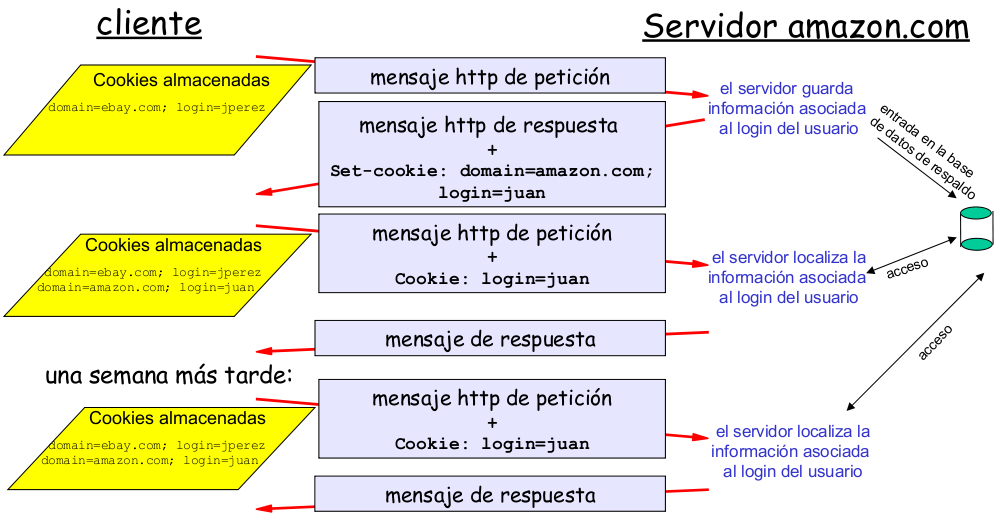
\includegraphics[width=1.05\textwidth]{figs/5-p40}
\end{center}

\end{frame}

%%%%%%%%%%%%%%%%%%%%%%%%%%%%%%%%%%%%%%%%%%%%%%%%%%%%%%%%%%%%%%%%%%%





%%%%%%%%%%%%%%%%%%%%%%%%%%%%%%%%%%%%%%%%%%%%%%%%%%%%%%%%%%%%%%%%%%%
\section{HTTPS}
%%%%%%%%%%%%%%%%%%%%%%%%%%%%%%%%%%%%%%%%%%%%%%%%%%%%%%%%%%%%%%%%%%%


\begin{frame}[fragile]
\frametitle{HTTPS}

\begin{center}
\includegraphics[width=0.7\textwidth]{figs/https}  
\end{center}

\begin{itemize}
\item El término \res{HTTPS} se refiere a colocar HTTP sobre \res{TLS} \emph{(Transport Layer Security)}.
\item TLS aporta características de seguridad a las conexiones
  TCP. Antiguamente se llamaba SSL \emph{(Secure Sockets Layer)}
\item Permite confidencialidad en la conexión (mediante cifrado),
  autenticación de los extremos e integridad del contenido.
\item Las URLs comienzan por \textcolor{darkblue}{\Verb|https://|}
\end{itemize}

\end{frame}




%%%%%%%%%%%%%%%%%%%%%%%%%%%%%%%%%%%%%%%%%%%%%%%%%%%%%%%%%%%%%%%%%%%
\section{HTTP 2.0}
%%%%%%%%%%%%%%%%%%%%%%%%%%%%%%%%%%%%%%%%%%%%%%%%%%%%%%%%%%%%%%%%%%%


%%%%%%%%%%%%%%%%%%%%%%%%%%%%%%%%%%%%%%%%%%%%%%%%%%%%%%%%%%%%%%%%%%%

\begin{frame}[fragile]
\frametitle{HTTP 2.0}


\begin{itemize}
\item \res{HTTP/2.0} será la nueva versión de HTTP.
\item Principales características:
  \begin{itemize}
  \item Se mantiene la semántica de HTTP/1.1 en cuanto a métodos,
    códigos de respuesta, URLs, cabeceras\ldots
  \item Se especifica cómo será la interación entre clientes 1.1 y
    servidores 2.0 o viceversa
  \item Una sola conexión para transmitir todos los recursos del mismo
    servidor, cada petición/respuesta de un recurso será un flujo
    \emph{(stream)} dentro de la conexión
  \item Cabeceras binarias (no de texto), mediante compresión (el tamaño
    medio de cabeceras en 1.1: 800 bytes (!!!)).
  \item Paquetes de datos y paquetes de control
  \item Prioridades en los flujos para evitar tener que esperar a
    completar los recursos previos para que llegue un recurso
    imprescindible para ir mostrando todo el contenido.
  \item Sobre TLS.
  \item Extensible para poder cubrir futuras necesidades.
  \end{itemize}
\end{itemize}

\end{frame}



%%%%%%%%%%%%%%%%%%%%%%%%%%%%%%%%%%%%%%%%%%%%%%%%%%%%%%%%%%%%%%%%%%%

\begin{frame}[fragile]
\frametitle{SPDY}


\begin{itemize}
\item HTTP/2.0 está basado (como punto de partida) en el protocolo \res{SPDY}.
\item SPDY es un protocolo desarrollado por Google para reemplazar
  HTTP de forma más eficiente.
  \begin{itemize}
  \item SPDY se puede usar hoy
  \item Reduce el tiempo de carga de página un 65\% utilizando flujos,
    compresión y formato binario de paquetes.
  \item Necesita clientes y servidores que lo soporten:
    \begin{itemize}
    \item Clientes: Chrome, Firefox 13+, Opera 12.10+, Explorer 11+
    \item Servidores: Todas las aplicaciones web de Google, Twitter,
      Facebook, Wordpress\ldots
    \item \verb|http://spdycheck.org/| para comprobar si un sitio
      soporta SPDY. 
    \end{itemize}
  \end{itemize}
\end{itemize}

\end{frame}




%%%%%%%%%%%%%%%%%%%%%%%%%%%%%%%%%%%%%%%%%%%%%%%%%%%%%%%%%%%%%%%%%%%
\section{Referencias}
%%%%%%%%%%%%%%%%%%%%%%%%%%%%%%%%%%%%%%%%%%%%%%%%%%%%%%%%%%%%%%%%%%%

\begin{frame}[fragile,shrink=8]
\frametitle{Referencias}


\begin{itemize}

\item J.J. Kurose y K.W. Ross, \textbf{Redes de Computadores: un
    enfoque descendente basado en Internet}, Pearson Educación, 2ª
  edición.

\item W. Richard Stevens, \textbf{TCP/IP Illustrated, vol 3}, Addisson
  Wesley.

\item James Marshall, \textbf{HTTP Made Really Easy. A Practical Guide to Writing Clients and Servers}, \Verb|http://www.jmarshall.com/easy/http/|

\item RFC 1945, \textbf{HTTP 1.0},
  \verb|http://www.faqs.org/rfcs/rfc1945.html| 
\item RFC 2068, \textbf{HTTP 1.1},
  \verb|http://www.faqs.org/rfcs/rfc2068.html| 
\item RFC 7540, \textbf{HTTP 2.0},
  \verb|http://www.faqs.org/rfcs/rfc7540.html| 
\item RFC 2964, \textbf{Use of HTTP State Management},
  \verb|http://www.faqs.org/rfcs/rfc2964.html| 
\item RFC 2965, \textbf{HTTP State Management Mechanism},
  \verb|http://www.faqs.org/rfcs/rfc2965.html| 


\end{itemize}

\end{frame}


%%%%%%%%%%%%%%%%%%%%%%%%%%%%%%%%%%%%%%%%%%%%%%%%%%%%%%%%%%%%%%%%%%%


\end{document}





%%% Local Variables: 
%%% mode: latex
%%% TeX-master: t
%%% End: 
